\documentclass[conference]{IEEEtran}
\IEEEoverridecommandlockouts
\usepackage{cite}
\usepackage{graphicx}
\usepackage{xcolor}
\usepackage{booktabs}
\usepackage{amsmath}
\usepackage{tikz}
\usepackage{hyperref}
\usetikzlibrary{arrows.meta,positioning,fit}

\begin{document}

\title{AuraSync: An Audio Intelligence System for Visual Knowledge Extraction}

\author{
  \IEEEauthorblockN{Smitha M}
  \IEEEauthorblockA{\textit{CHRIST (Deemed to be University)}\\
  Bangalore, India \\
  smitha.m@msam.christuniversity.in}
  \and
  \IEEEauthorblockN{Dr. Rupali Sunil Wagh}
  \IEEEauthorblockA{\textit{CHRIST (Deemed to be University)}\\
  Bangalore, India\\
  rupali.wagh@christuniversity.in}
  \and
  \IEEEauthorblockN{Dr. Helen K Joy}
  \IEEEauthorblockA{\textit{CHRIST (Deemed to be University)}\\
  Bangalore, India\\
  helenk.joy@christuniversity.in}
}

\maketitle

\begin{abstract}
Audio recordings contain decisions, actions, and quantitative information that are difficult to revisit in a long transcript. AuraSync is a full-stack application that converts uploaded recordings into transcripts, speaker-oriented analysis, structured topic and metric data, and visual outputs. This paper describes the repository's FastAPI implementation: audio ingestion and transcription feed a LangGraph-based analysis pipeline, whose flow, speaker, and metric agents execute concurrently before a knowledge-tree assembler generates positioned nodes and exportable artifacts. The React client uses an asynchronous job API, while a separate direct-analysis route returns tree and export data; the job adapter currently has a result-schema mapping gap. The repository also contains a legacy Node.js backend, which is not described here. Because the project does not include a labeled evaluation corpus or controlled baseline, this paper reports architecture and available functional testing rather than unsupported accuracy or latency claims.
\end{abstract}

\begin{IEEEkeywords}
audio intelligence, speech transcription, language models, multi-agent systems, knowledge visualization
\end{IEEEkeywords}

\section{Introduction}
Meetings, lectures, and interviews produce information that is easy to record but costly to review. A transcript improves searchability, yet a reader must still identify discussion structure, speakers, evidence, and follow-up actions. Meeting-summary datasets such as QMSum and MeetingBank formalize related summarization tasks and provide human-authored reference material for evaluation \cite{qmsum,meetingbank}. AuraSync addresses a complementary systems problem: connecting transcription and structured extraction to a persistent, reviewable visual result.

This paper documents the Python/FastAPI implementation in the project repository and its React client. It focuses on asynchronous job processing, Whisper-based transcription, concurrent language-model analysis, knowledge-tree assembly, export generation, and a polling interface. The separate legacy Node.js backend is not treated as part of the described system. Nor do we make quantitative quality claims: the repository contains no annotated benchmark dataset or controlled baseline.

Prior work informs the separate tasks in this system. Transformer and self-supervised approaches provide context for contemporary speech recognition \cite{attention,wav2vec,speechtransformer,whisper}; BART, T5, and multi-stage methods address abstractive and long-input summarization \cite{bart,t5,summn}. Meeting corpora such as AMI, QMSum, and MeetingBank illustrate the annotation needed for empirical comparisons \cite{ami,qmsum,meetingbank}. Agent frameworks motivate decomposing a complex request into specialized operations, although their results do not establish that this particular pipeline is more accurate \cite{agentsurvey,react,autogen}. Long-context and hallucination studies further motivate treating generated content as reviewable suggestions rather than ground truth \cite{longcontext,hallucinationsurvey,halueval}. Dedicated acoustic diarization systems are a useful contrast to AuraSync's transcript-derived speaker processing \cite{pyannote,fujita}.

\section{System Overview}
AuraSync comprises a React 18 and Vite frontend and a Python service built with FastAPI. The primary client path submits authenticated jobs and polls status and result endpoints. A separate audio-analysis route accepts an upload and returns a knowledge-tree result and export metadata directly. Audio processing and analysis run on the backend; the browser presents generated results rather than performing inference. The framework documentation describes these implementation dependencies, not a performance guarantee for AuraSync \cite{fastapi,reactdocs,langgraphdocs,plotlydocs}.

Fig.~\ref{fig:architecture} summarizes the implemented processing path. After transcription, the analysis graph executes flow, speaker, and metric tasks concurrently. Their outputs are assembled into a positioned knowledge tree and passed to the export service. Job status advances through processing stages so the client can show progress and retrieve completed results.

\begin{figure*}[t]
\centering
\resizebox{0.96\textwidth}{!}{%
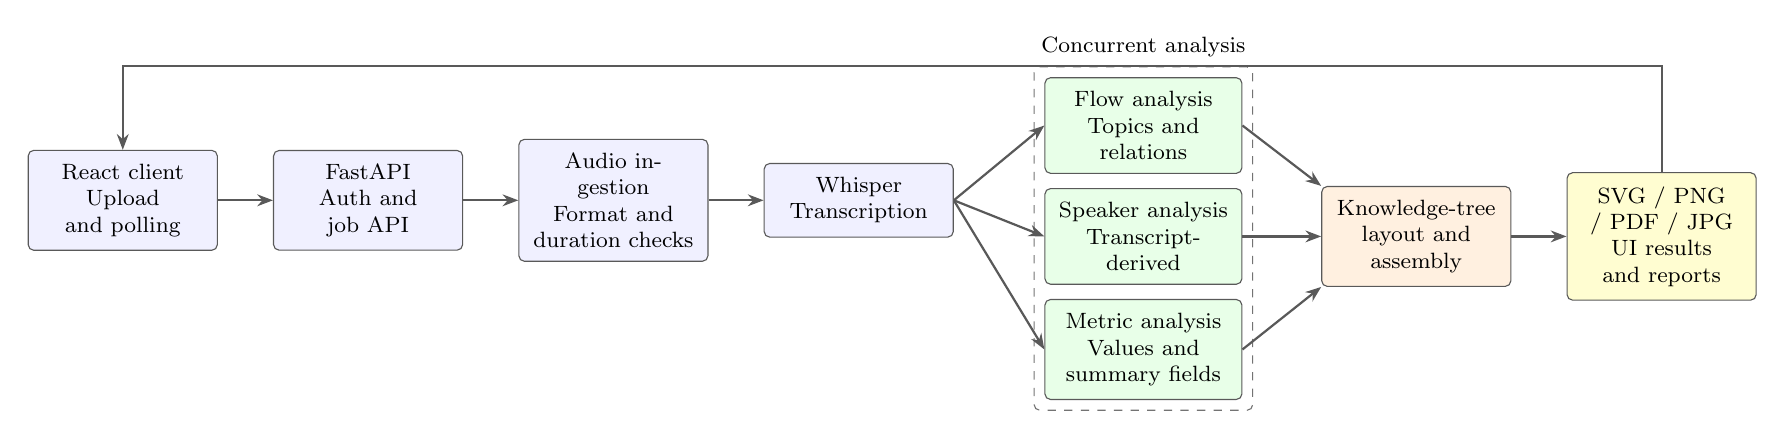
\begin{tikzpicture}[
  box/.style={draw=black!65, rounded corners=2pt, fill=blue!6,
    minimum height=0.9cm, text width=2.05cm, align=center,
    font=\footnotesize, inner sep=5pt},
  agent/.style={box, fill=green!9, text width=2.15cm},
  arrow/.style={-{Stealth[length=2mm]}, thick, draw=black!65},
  node distance=0.55cm and 0.7cm
]
\node[box] (client) {React client\\Upload and polling};
\node[box, right=of client] (api) {FastAPI\\Auth and job API};
\node[box, right=of api] (ingest) {Audio ingestion\\Format and duration checks};
\node[box, right=of ingest] (whisper) {Whisper\\Transcription};
\node[agent, right=1.15cm of whisper, yshift=0.95cm] (flow) {Flow analysis\\Topics and relations};
\node[agent, below=0.18cm of flow] (speaker) {Speaker analysis\\Transcript-derived};
\node[agent, below=0.18cm of speaker] (metrics) {Metric analysis\\Values and summary fields};
\node[draw=black!55, rounded corners=2pt, dashed, fit=(flow)(speaker)(metrics),
  inner sep=0.13cm, label={[font=\footnotesize]above:Concurrent analysis}] (agents) {};
\node[box, right=1.0cm of speaker, fill=orange!12] (assemble) {Knowledge-tree\\layout and assembly};
\node[box, right=of assemble, fill=yellow!18] (output) {SVG / PNG / PDF / JPG\\UI results and reports};
\draw[arrow] (client) -- (api);
\draw[arrow] (api) -- (ingest);
\draw[arrow] (ingest) -- (whisper);
\draw[arrow] (whisper.east) -- (flow.west);
\draw[arrow] (whisper.east) -- (speaker.west);
\draw[arrow] (whisper.east) -- (metrics.west);
\draw[arrow] (flow.east) -- (assemble.north west);
\draw[arrow] (speaker.east) -- (assemble.west);
\draw[arrow] (metrics.east) -- (assemble.south west);
\draw[arrow] (assemble) -- (output);
\draw[arrow] (output.north) -- ++(0,1.35) -| (client.north);
\end{tikzpicture}%
}
\caption{AuraSync processing and result-delivery path. Analysis branches run concurrently; completed outputs are assembled and returned to the client.}
\label{fig:architecture}
\end{figure*}

\section{Processing Pipeline}
\subsection{Ingestion and Transcription}
The ingestion stage accepts configured audio formats, checks the extension, size, and basic container signatures, and estimates duration. It prefers FFmpeg/ffprobe when available and uses format-specific or file-size estimates as fallback; therefore duration limits depend on the accuracy of the available probe. The job route applies the configured free-tier duration limit before transcription and rejects uploads above the configured size ceiling. These are application checks rather than a claim of exhaustive media-file security validation.

The transcription service uses OpenAI Whisper \cite{whisper}; the repository defaults to the \texttt{base} model on CPU. When FFmpeg is available, audio longer than the configured chunk duration is converted into chunks and transcribed concurrently up to a configured limit; returned text is merged in chronological chunk order. The default settings specify five-minute chunks and at most four parallel chunks. If the model cannot be loaded, the service returns a fixed demonstration transcript so that downstream paths can be exercised. That fallback is synthetic, not a transcript inferred from the uploaded recording, and must be excluded from any real-audio quality result.

\subsection{Concurrent Analysis}
The pipeline receives a transcript and constructs a LangGraph state. Decomposing analysis into specialized tasks follows broader work on language-model agents \cite{agentsurvey}. It first estimates speaker metadata from the transcript and optional speaker labels; this step does not process acoustic speaker embeddings. It then runs three prompt-driven tasks concurrently:
\begin{itemize}
  \item The flow agent extracts topic structure and relationships suitable for a flowchart or knowledge tree.
  \item The speaker agent produces speaker-oriented analysis from the transcript and speaker information.
  \item The metric agent extracts quantitative information and summary fields.
\end{itemize}
The flow output requests a root topic, short node labels, node categories, priority and confidence fields, speaker attribution, parent links, and typed relations. The speaker task requests topics, agreement and conflict pairs, and a node-to-speaker map. The metric task requests values with units and context, time series, timeline entries, a short title, tags, and an executive summary. Transcript input to these LLM tasks is sliced to the configured prefix length, 8,000 characters by default; this can omit later discussion content for longer recordings. Flow nodes and edges are normalized, invalid relationship endpoints are filtered, labels and priorities are bounded, and generated data is supplemented with fallback structures when required. These transformations improve shape consistency but do not verify semantic correctness.

After the parallel tasks finish, the assembler lays out tree nodes and edges and invokes the export service. Speaker statistics are derived separately from the transcript and supplied duration; they should not be interpreted as acoustic diarization or measured speaker-attribution accuracy.

\subsection{Knowledge-Tree Output}
The backend represents visual content as a rooted hierarchy of typed nodes and relationships. The layout engine identifies a root, attaches children using parent links and edges, assigns depth levels, estimates subtree widths, and places each node within a horizontal interval. Let $w_v$ be a node's width, $g$ the minimum gap, $C(v)$ its child set, $\ell(v)$ its depth, and $h$ the configured level height. The subtree width and vertical position are:
\begin{equation}
\begin{aligned}
S(v)&=\max\left(w_v+g,\sum_{c\in C(v)}S(c)\right),\\
y_v&=y_0+\ell(v)h.
\end{aligned}
\end{equation}
Child intervals are distributed in proportion to their subtree widths. This deterministic hierarchical layout is distinct from force-directed graph drawing \cite{graphdrawing,fruchterman}. Fig.~\ref{fig:tree} is a schematic example, not a screenshot or an output from a benchmark recording. The export service generates SVG and can render PNG, JPG, and PDF; the React application presents its separate mind-map, flowchart, and dashboard views.

\begin{figure}[t]
\centering
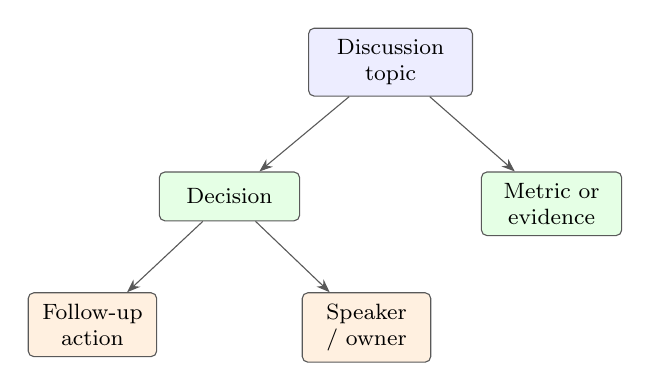
\begin{tikzpicture}[
  item/.style={draw=black!65, rounded corners=2pt, fill=blue!7,
    text width=1.8cm, align=center, font=\footnotesize, minimum height=0.62cm,
    inner sep=4pt},
  child/.style={item, fill=green!10, text width=1.5cm},
  leaf/.style={item, fill=orange!12, text width=1.35cm},
  link/.style={-{Stealth[length=1.7mm]}, draw=black!65}
]
\node[item] (root) {Discussion topic};
\node[child, below left=0.95cm and 0.1cm of root] (decision) {Decision};
\node[child, below right=0.95cm and 0.1cm of root] (evidence) {Metric or evidence};
\node[leaf, below left=0.9cm and 0.02cm of decision] (action) {Follow-up action};
\node[leaf, below right=0.9cm and 0.02cm of decision] (owner) {Speaker / owner};
\draw[link] (root) -- (decision);
\draw[link] (root) -- (evidence);
\draw[link] (decision) -- (action);
\draw[link] (decision) -- (owner);
\end{tikzpicture}
\caption{Schematic knowledge-tree structure showing topic, decision, evidence, and action relationships.}
\label{fig:tree}
\end{figure}

\section{Application Implementation}
\subsection{API and Job Lifecycle}
The FastAPI application exposes the authenticated job workflow used by the frontend. Table~\ref{tab:api} summarizes its principal endpoints and the separate direct-analysis route. Upload validation checks the requested output mode, supported extension, file size, and speaker-count range before creating a job associated with the authenticated user. The job store persists status and intermediate fields to MongoDB when available and otherwise falls back to process-local memory. Authentication, report, user, and subscription routes support the surrounding application.

\begin{table}[t]
\caption{Job and Direct Audio API Endpoints}
\label{tab:api}
\centering
\scriptsize
\begin{tabular}{@{}p{0.53\columnwidth}p{0.40\columnwidth}@{}}
\toprule
\textbf{Endpoint} & \textbf{Purpose} \\
\midrule
\shortstack[l]{\texttt{POST /api/v1/jobs/upload}} & Submit audio and options \\
\shortstack[l]{\texttt{GET /api/v1/jobs/}\\\texttt{\{id\}/status}} & Read stage and partial results \\
\shortstack[l]{\texttt{GET /api/v1/jobs/}\\\texttt{\{id\}/result}} & Retrieve completed result \\
\shortstack[l]{\texttt{POST /api/audio/}\\\texttt{analyze-and-generate-tree}} & Direct tree analysis and exports \\
\bottomrule
\end{tabular}
\end{table}

A job progresses through pending, transcription, diarization, analysis, visualization, summarization, and completion, or enters a failed state with an error. The upload handler launches processing as an in-process asynchronous task; Mongo persistence does not by itself provide a durable external work queue. The browser polls status and requests the final result when processing completes. This is asynchronous job handling, not streaming or real-time inference.

\subsection{Model Configuration and Fallbacks}
The Python backend uses one configurable OpenAI-compatible chat-completions endpoint, rather than the multi-provider Groq/Google/Together routing described in the earlier draft. The default model name is \texttt{gpt-4o-mini}; a non-empty API key enables remote inference, while the default empty key or demo mode selects offline generators. Requests use JSON response mode, a configurable temperature (default 0.2), and a bounded retry loop (default two attempts). When requests fail or no key is configured, deterministic templates return fixed example structures. These responses demonstrate schema flow but are not content-grounded analysis of the uploaded recording. Metric extraction also includes regex patterns for currencies, percentages, dates, and deadline language when the model output omits metrics; if no matches exist, its final fallback supplies example values. Consequently, evaluation must record the inference mode and separate real-model results from demonstration or rule-based output.

\subsection{Client and Deployment Modes}
The React client offers mind-map, flowchart, and dashboard views and a reports workflow. The Python backend can use configured external model services; its documentation also describes deterministic/offline and demo fallbacks for development. Fallback output helps exercise the application path, but must be distinguished from output produced by the intended speech and language models in any scientific evaluation.

The repository contains a separate Node.js/Express backend with overlapping functionality. To keep the system description reproducible, this paper concerns \texttt{backend-py}; deployments should select one backend and configure the frontend API base URL accordingly. The Node backend is not evidence for behavior attributed to the Python pipeline.

\section{Verification and Evaluation Scope}
The repository has complementary functional checks. Unit tests exercise speaker metadata extraction, each analysis agent, tree positioning, and SVG/PNG/JPG/PDF export generation. A route test submits a short generated WAV to the direct analysis endpoint and checks the response, analysis identifier, and SVG download path. The smoke script exercises account creation, authenticated job upload, polling, report operations, error handling, and a subscription-limit case. These checks establish that selected application paths can be exercised; the generated waveform and deterministic fallback are not a labeled audio corpus, and assertions on response shape do not measure semantic correctness, transcription quality, or comparative model performance.

The repository does not supply a labeled audio corpus, annotation protocol, repeated-trial results, or reproducible monolithic baseline. Existing meeting corpora illustrate the value of documented references for summarization evaluation \cite{ami,qmsum,meetingbank,summn}. Accordingly, this paper does not report success rates, word error rate, diarization accuracy, latency per audio hour, schema adherence, provider-failover percentages, or cost savings. Hallucination benchmarks likewise emphasize the need for task-specific, labeled evaluation \cite{halueval}. A quantitative study would need a documented dataset and consent/privacy process, reference transcripts and labels, task-specific metrics, hardware and model configuration, repeated runs, and baseline prompts and costs.

\section{Limitations and Future Work}
Transcript-derived speaker processing cannot reliably resolve speaker turns or overlap in the way an acoustic diarization model can; dedicated neural diarization systems address that separate task \cite{pyannote,fujita}. Output quality also depends on transcription quality, model configuration, transcript length, and fallback mode; long-context models can still exhibit position-sensitive information use \cite{longcontext}, and generated content can contain unsupported claims \cite{hallucinationsurvey,halueval}. The project does not yet provide a human-labeled quality study or calibrated confidence. There is also an integration gap in the queued job path: the analysis assembler returns \texttt{knowledgeTree} and \texttt{exports}, whereas the job orchestrator currently reads \texttt{visual} and \texttt{metrics}; the job schema can therefore complete without storing the generated visual payload. The direct audio-analysis endpoint does return the tree and exports, but it is a distinct route. Mapping these result contracts and adding an assertion that the queued result contains renderable nodes and edges are prerequisites for claiming complete end-to-end visualization through job polling. The two backend implementations create a further reproducibility risk unless the selected implementation and configuration are recorded for each deployment and experiment. Automated extraction can omit, merge, or misattribute information, so results should be reviewed before being treated as authoritative records.

Future work should prioritize evaluation on a consented, representative audio set with human-reviewed transcripts, speaker labels, decisions, actions, and topic relations. Retrieval-augmented processing is another candidate for long recordings, but is not implemented here \cite{rag}. Other directions include acoustic diarization, confidence calibration against labeled data, and recording the model, configuration, runtime, and fallback mode for each run. Streaming or multimodal processing should be treated as future work, not as a current capability.

\section{Conclusion}
AuraSync combines transcription, concurrent language-model analysis, knowledge-tree assembly, export generation, and a polling-based React interface. This paper describes the repository's FastAPI implementation and distinguishes its workflow from the legacy Node backend. The system provides an extensible engineering foundation; its scientific performance remains an open question until a reproducible, labeled evaluation is conducted.

\begin{thebibliography}{00}
\bibitem{whisper}
A. Radford \emph{et al.}, ``Robust Speech Recognition via Large-Scale Weak Supervision,'' in \emph{Proc. 40th Int. Conf. Machine Learning}, PMLR, vol. 202, 2023, pp. 28492--28518.

\bibitem{qmsum}
M. Zhong \emph{et al.}, ``QMSum: A New Benchmark for Query-based Multi-domain Meeting Summarization,'' in \emph{Proc. NAACL-HLT}, 2021, pp. 5905--5921.

\bibitem{agentsurvey}
X. Wang \emph{et al.}, ``A Survey on Large Language Model based Autonomous Agents,'' arXiv:2308.11432, 2023.

\bibitem{rag}
P. Lewis \emph{et al.}, ``Retrieval-Augmented Generation for Knowledge-Intensive NLP Tasks,'' in \emph{Advances in Neural Information Processing Systems}, vol. 33, 2020, pp. 9459--9474.

\bibitem{attention}
A. Vaswani \emph{et al.}, ``Attention Is All You Need,'' in \emph{Advances in Neural Information Processing Systems}, vol. 30, 2017.

\bibitem{wav2vec}
A. Baevski, Y. Zhou, A. Mohamed, and M. Auli, ``wav2vec 2.0: A Framework for Self-Supervised Learning of Speech Representations,'' in \emph{Advances in Neural Information Processing Systems}, vol. 33, 2020, pp. 12449--12460.

\bibitem{speechtransformer}
L. Dong, S. Xu, and B. Xu, ``Speech-Transformer: A No-Recurrence Sequence-to-Sequence Model for Speech Recognition,'' in \emph{Proc. IEEE Int. Conf. Acoustics, Speech and Signal Processing}, 2018, pp. 5884--5888.

\bibitem{ami}
J. Carletta \emph{et al.}, ``The AMI Meeting Corpus: A Pre-announcement,'' in \emph{Machine Learning for Multimodal Interaction}, Lecture Notes in Computer Science, vol. 3869, 2005, pp. 28--39.

\bibitem{meetingbank}
Y. Hu \emph{et al.}, ``MeetingBank: A Benchmark Dataset for Meeting Summarization,'' in \emph{Proc. 61st Annu. Meeting of the Association for Computational Linguistics}, 2023, pp. 16409--16423.

\bibitem{summn}
Y. Zhang \emph{et al.}, ``Summ$^N$: A Multi-Stage Summarization Framework for Long Input Dialogues and Documents,'' in \emph{Proc. 60th Annu. Meeting of the Association for Computational Linguistics}, 2022, pp. 1592--1604.

\bibitem{bart}
M. Lewis \emph{et al.}, ``BART: Denoising Sequence-to-Sequence Pre-training for Natural Language Generation, Translation, and Comprehension,'' in \emph{Proc. 58th Annu. Meeting of the Association for Computational Linguistics}, 2020, pp. 7871--7880.

\bibitem{t5}
C. Raffel \emph{et al.}, ``Exploring the Limits of Transfer Learning with a Unified Text-to-Text Transformer,'' \emph{J. Machine Learning Research}, vol. 21, no. 140, pp. 1--67, 2020.

\bibitem{react}
S. Yao \emph{et al.}, ``ReAct: Synergizing Reasoning and Acting in Language Models,'' in \emph{Proc. Int. Conf. Learning Representations}, 2023.

\bibitem{autogen}
Q. Wu \emph{et al.}, ``AutoGen: Enabling Next-Gen LLM Applications via Multi-Agent Conversation,'' arXiv:2308.08155, 2023.

\bibitem{longcontext}
N. F. Liu \emph{et al.}, ``Lost in the Middle: How Language Models Use Long Contexts,'' \emph{Trans. Assoc. Comput. Linguistics}, vol. 12, pp. 157--173, 2024.

\bibitem{hallucinationsurvey}
Z. Ji \emph{et al.}, ``Survey of Hallucination in Natural Language Generation,'' \emph{ACM Computing Surveys}, vol. 55, no. 12, Article 248, 2023.

\bibitem{halueval}
J. Li \emph{et al.}, ``HaluEval: A Large-Scale Hallucination Evaluation Benchmark for Large Language Models,'' in \emph{Proc. Conf. Empirical Methods in Natural Language Processing}, 2023, pp. 6449--6464.

\bibitem{pyannote}
H. Bredin \emph{et al.}, ``pyannote.audio: Neural Building Blocks for Speaker Diarization,'' in \emph{Proc. IEEE Int. Conf. Acoustics, Speech and Signal Processing}, 2020.

\bibitem{fujita}
Y. Fujita \emph{et al.}, ``End-to-End Neural Speaker Diarization with Permutation-Free Objectives,'' in \emph{Proc. Interspeech}, 2019, pp. 4300--4304.

\bibitem{fruchterman}
T. M. J. Fruchterman and E. M. Reingold, ``Graph Drawing by Force-Directed Placement,'' \emph{Software: Practice and Experience}, vol. 21, no. 11, pp. 1129--1164, 1991.

\bibitem{graphdrawing}
R. Tamassia, Ed., \emph{Handbook of Graph Drawing and Visualization}. Boca Raton, FL, USA: CRC Press, 2013.

\bibitem{fastapi}
FastAPI, ``FastAPI Documentation.'' [Online]. Available: \url{https://fastapi.tiangolo.com/}. Accessed: Sep. 27, 2026.

\bibitem{reactdocs}
Meta Open Source, ``React Documentation.'' [Online]. Available: \url{https://react.dev/}. Accessed: Sep. 27, 2026.

\bibitem{langgraphdocs}
LangChain, ``LangGraph Overview.'' [Online]. Available: \url{https://docs.langchain.com/oss/python/langgraph/overview}. Accessed: Sep. 27, 2026.

\bibitem{plotlydocs}
Plotly Technologies Inc., ``Plotly Open Source Graphing Library for Python.'' [Online]. Available: \url{https://plotly.com/python/}. Accessed: Sep. 27, 2026.
\end{thebibliography}

\end{document}
